\documentclass[11pt,letterpaper]{article}

% ─── Packages ─────────────────────────────────────────────────────
\usepackage[utf8]{inputenc}
\usepackage[T1]{fontenc}
\usepackage{amsmath,amssymb}
\usepackage[margin=0.7in]{geometry}
\usepackage{graphicx}
\usepackage{xcolor}
\usepackage{titlesec}
\usepackage{caption}
\usepackage{enumitem}
\usepackage[expansion=false]{microtype}
\usepackage[hidelinks]{hyperref}
\usepackage{parskip}
\usepackage{booktabs}

% ─── Colors ───────────────────────────────────────────────────────
\definecolor{HeadColor}{HTML}{1A1F36}
\definecolor{AccentColor}{HTML}{1F4E8C}
\definecolor{MutedColor}{HTML}{6B7280}
\definecolor{BodyColor}{HTML}{1F2937}

% ─── Heading style ────────────────────────────────────────────────
\titleformat{\section}
  {\color{HeadColor}\normalfont\large\bfseries}
  {\thesection.}{0.35em}{}
\titleformat{\subsection}
  {\color{HeadColor}\normalfont\normalsize\bfseries}
  {\thesubsection}{0.35em}{}
\titlespacing*{\section}{0pt}{8pt}{2pt}
\titlespacing*{\subsection}{0pt}{6pt}{1pt}

% Caption style
\captionsetup{font={small,it,color=MutedColor},labelfont={bf,color=MutedColor},skip=2pt}

% Paragraph spacing
\setlength{\parskip}{1.5pt plus 0.5pt}
\setlength{\parindent}{0pt}
\linespread{1.01}

% Default text color
\AtBeginDocument{\color{BodyColor}}

% Suppress page numbers
\pagestyle{empty}

% Hanging indent for references
\newcommand{\refitem}[1]{%
  \par\noindent\hangindent=2em\hangafter=1 \small #1\par%
}

% ═══════════════════════════════════════════════════════════════════
\begin{document}

% ─── Title block ──────────────────────────────────────────────────
\begin{center}
  {\Large\bfseries\color{HeadColor} Probing Visual Affordance Across Two Robotic Visual Pipelines}\par
  \vspace{2pt}
  {\itshape\color{MutedColor}\normalsize VLA encoders ($\pi_0$, $\pi_{0.5}$) and generative diffusion models (Flux) on UMD and AGD20K}\par
  \vspace{4pt}
  {\color{AccentColor}\small Aleks Antari \quad\textperiodcentered\quad Nitik Jain \quad\textperiodcentered\quad Spring 2026}\par
\end{center}
\vspace{-4pt}
\noindent\textcolor{AccentColor}{\rule{\linewidth}{0.5pt}}
\vspace{-2pt}

% ─── 1. Introduction ─────────────────────────────────────────────
\section{Introduction}

Modern robot policies route visual information through one of two architectural paradigms. \textbf{Vision–Language–Action (VLA)} models such as $\pi_0$ [1] and $\pi_{0.5}$ [2] fine-tune a contrastive SigLIP encoder [3] inside a PaliGemma backbone [4] toward action prediction. \textbf{Generative world-model policies} (e.g. Cosmos Predict2) instead use language-conditioned image/video diffusion to predict future states, and recent work [5] has shown that the cross-attention layers in such diffusion models encode \emph{verb-spatial binding}: text tokens like ``cut'' or ``pour'' activate spatially specific regions of the generated scene without ever being trained to do so.

These two paradigms process language and vision in opposite ways. VLAs are \textbf{image-conditioned language models} --- the visual encoder is pushed toward action-token prediction. World-model policies are \textbf{language-conditioned image models} --- text drives spatial generation through cross-attention. If both perceptual loops carry useful affordance signal, they may carry \emph{different kinds} of it. The goal of Phase 1 is to characterize that difference empirically, using probing methods that hold all measurement protocols fixed.

We pursue two complementary axes. \textbf{Axis 1} (\S\ref{sec:axis1}) probes the SigLIP encoder along the VLA fine-tuning trajectory ($\text{raw}\to\text{PaliGemma}\to\pi_0\to\pi_{0.5}$) with linear probing on UMD [6]. \textbf{Axis 2} (\S\ref{sec:axis2}) extracts cross-attention maps from FLUX.1 [7] during denoising and measures verb-spatial binding on AGD20K [8].

% ─── 2. Method ───────────────────────────────────────────────────
\section{Method}

\subsection{Axis 1 — linear probing of VLA-stage SigLIP variants on UMD}
We adapt the geometry probe of [5]: each encoder is frozen; four equally-spaced intermediate transformer layers are hooked, fused by bilinear resize + channel concat, and a BatchNorm--$1{\times}1$ Conv head predicts the seven UMD affordance classes (\emph{grasp/cut/scoop/contain/pound/support/w-grasp}). Patches are scored at the patch-grid resolution (majority-vote, $\geq 55\%$ coverage); evaluation by mIoU on UMD's category-split test set. Each (encoder, resolution) cell is run at \textbf{n{=}4 seeds}. Pipeline validation: DINOv2-B at UMD-native reproduces $0.666$ mIoU vs the $0.670$ reported in [5]. We probe six encoders --- DINOv2-B/L [9] and four SigLIP-So400m stages (raw, PaliGemma stage-1, $\pi_0$, $\pi_{0.5}$) --- at two resolutions: \textbf{res224} ($16{\times}16$ patches, the VLA's operating resolution) and \textbf{resumd} (UMD-native ${\sim}480{\times}640$, $35{\times}46$ patches).

\subsection{Axis 2 — verb-spatial binding via cross-attention extraction on FLUX.1}
For each AGD20K image+verb pair we generate from FLUX.1 with the prompt \texttt{``a person \{verb\} a \{object\}''}, registering a custom \texttt{AttentionProcessor} on every \texttt{FluxTransformerBlock.attn} module to record the post-softmax image-query~$\times$~text-key slice (the diffusers-default processor uses scaled-dot-product attention which does not expose probabilities). After head-averaging and per-block aggregation across denoising timesteps, we obtain one verb-conditioned attention map per sample, upsample bilinearly to the GT resolution, and compute three standard saliency metrics against AGD20K's GT heatmaps: \textbf{KLD} (lower is better), \textbf{SIM} (histogram intersection), and \textbf{NSS} (z-score of predicted map at the top-20\% GT pixels). We probe FLUX.1-schnell (4 steps, no CFG) and FLUX.1-dev (20 steps, CFG=3.5) on the full AGD20K egocentric set (\textbf{n{=}1675} across 36 affordance categories).

% ─── 3. Axis 1 — VLA encoder probing ─────────────────────────────
\section{Results — Axis 1: VLA encoder probing on UMD}
\label{sec:axis1}

\begin{figure}[h]
  \centering
  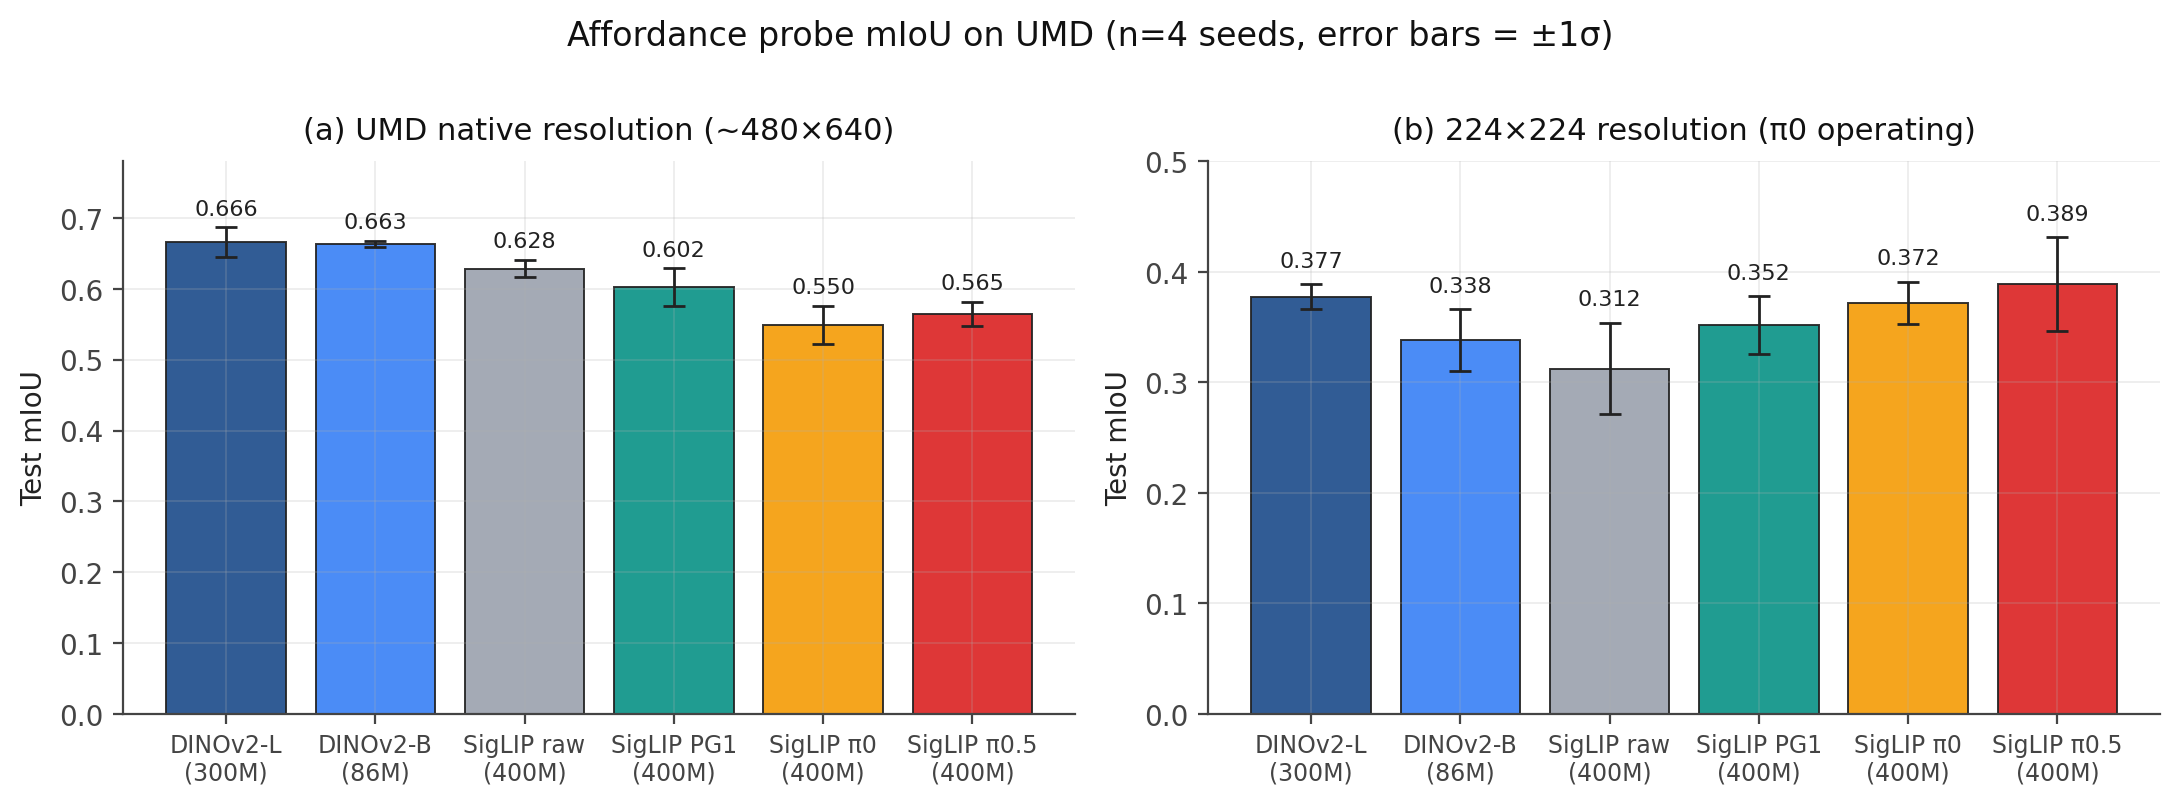
\includegraphics[width=0.97\linewidth]{fig1_bars.png}
  \caption{Test mIoU at both resolutions, n=4 seeds (error bars $\pm 1\sigma$). At UMD-native, DINOv2 dominates SigLIP at matched or smaller params; at the VLA operating resolution, encoder differences compress into seed noise.}
  \label{fig:bars}
\end{figure}

\textbf{Encoder rankings depend on resolution.} At UMD-native (Fig.~\ref{fig:bars}), both DINOv2 variants beat every SigLIP variant: DINOv2-B at 86M parameters outperforms SigLIP at 400M (+3.5 pp, exceeding either side's $\sigma$). This is the cleanest inter-encoder comparison in the project. At $224{\times}224$, five of six encoders cluster within 0.31--0.39 mIoU with overlapping error bars; only the top--bottom gap ($\pi_{0.5}$ vs raw, $\sim$7.6 pp) clearly survives.

\begin{figure}[h]
  \centering
  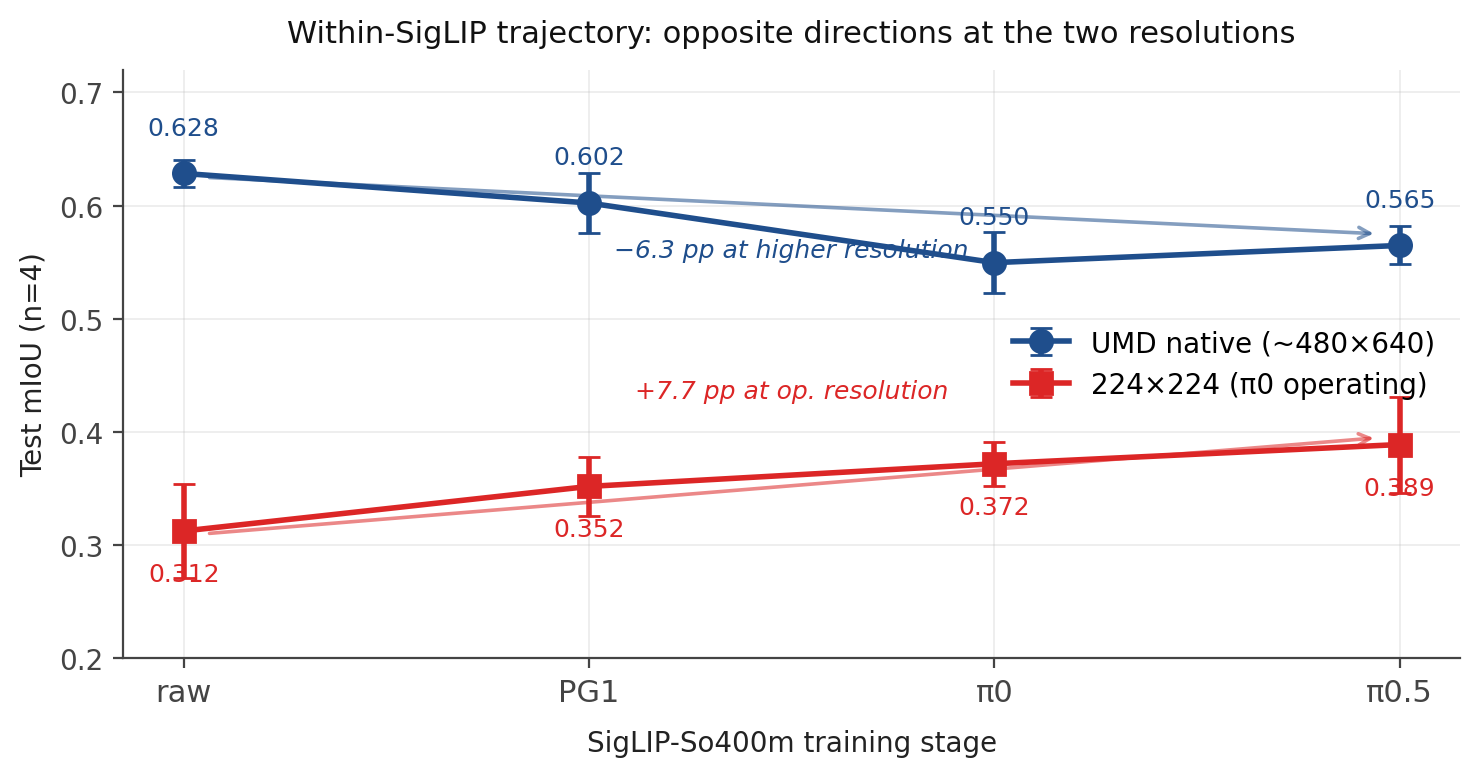
\includegraphics[width=0.62\linewidth]{fig2_trajectory.png}
  \caption{Within-SigLIP trajectory across training stages. VLA fine-tuning helps at the operating resolution and hurts at the higher UMD-native resolution.}
  \label{fig:trajectory}
\end{figure}

\textbf{The VLA trajectory reverses sign across resolutions.} Tracking the same 400M SigLIP across its four training stages (Fig.~\ref{fig:trajectory}): at \textbf{res224}, VLA fine-tuning helps monotonically (raw $0.31\to$ PG1 $0.35\to\pi_0$ $0.37\to\pi_{0.5}$ $0.39$, +7.7 pp cumulative); at \textbf{resumd}, it is net negative (raw $0.63\to$ PG1 $0.60\to\pi_0$ $0.55\to\pi_{0.5}$ $0.56$, $-6.3$ pp). VLA fine-tuning produces a \textbf{resolution-specialized} representation: gains at the training resolution, losses at higher resolution where the probe sees ${\sim}6\times$ more supervision signal per image. The $\Delta$(resumd $-$ res224) for VLA variants is roughly half what raw SigLIP and DINOv2 show ($+0.18$ vs $+0.30$), consistent with saturation at the training resolution.

\textbf{The probe is too coarse at the operating resolution to rank fine-grained differences} (n=4, $\sigma$ ranges 0.011--0.042 per cell, adjacent-rank gaps of 0.5--2.6 pp fall inside individual encoder noise). Single-seed encoder rankings at coarse patch grids should not be trusted.

% ─── 4. Axis 2 — generative-model verb-spatial binding ───────────
\section{Results — Axis 2: verb-spatial binding in FLUX.1}
\label{sec:axis2}

\begin{figure}[h]
  \centering
  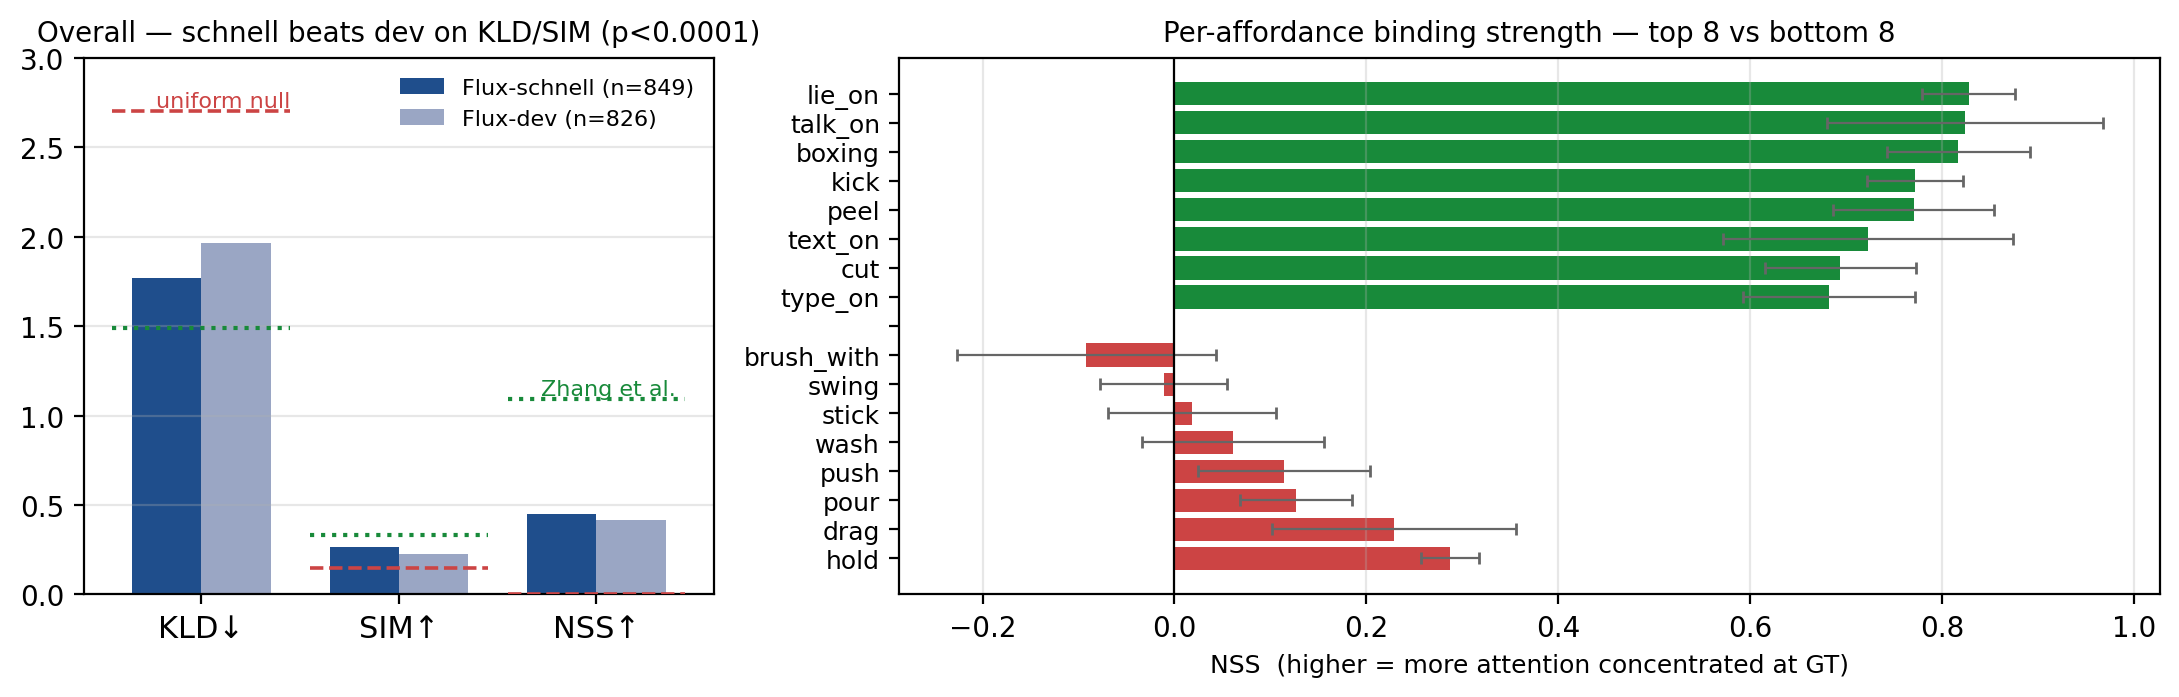
\includegraphics[width=0.99\linewidth]{fig3_axis2.png}
  \caption{(\textit{Left}) Overall metrics on AGD20K, n=1675. FLUX-schnell beats FLUX-dev significantly on KLD and SIM (Mann-Whitney $p<10^{-4}$); both sit well above uniform-null and below Zhang et al.'s published Flux numbers (green dotted). (\textit{Right}) Top 8 and bottom 8 affordances by NSS. Postural/contact verbs dominate; distributed actions cluster at zero.}
  \label{fig:axis2}
\end{figure}

\textbf{Verb-spatial binding is real and above null.} Across all 1675 samples, KLD $= 1.86$, SIM $= 0.25$, NSS $= +0.43$. The uniform-attention null gives KLD${\approx}2.7$, SIM${\approx}0.15$, NSS${=}0$. All three metrics depart from null in the expected direction (Fig.~\ref{fig:axis2}, left): KLD is 31\% below null, SIM is 67\% above null, NSS is half a standard deviation of GT-region concentration above zero. The qualitative claim --- that FLUX's cross-attention encodes verb-conditioned spatial structure aligned with affordance GT --- holds.

\textbf{Fast/sloppy beats slow/careful} (counterintuitive). FLUX-schnell (4 steps, no CFG) significantly beats FLUX-dev (20 steps, CFG=3.5) on KLD ($1.77$ vs $1.97$, $p<10^{-4}$) and SIM ($0.27$ vs $0.22$, $p<10^{-4}$); NSS is statistically indistinguishable ($p=0.16$). Five times more inference compute does not improve --- and in fact slightly degrades --- attention's alignment with GT. The likely mechanism: CFG amplifies the model's prompt-conditioned interpretation rather than what is in the image. Schnell's shorter trajectory stays closer to ``rough attention to actual content.'' \emph{Methodological implication}: cheap configurations are valid measurement tools for this kind of cross-attention probing.

\textbf{Manipulation verbs bind \emph{weaker} than non-manipulation verbs} (also counterintuitive). Stratifying by verb type, manipulation verbs (\textit{hold, push, lift, pour, pick\_up, cut, ...}) have mean NSS $= +0.349$ (n=794); other verbs (\textit{lie\_on, talk\_on, boxing, ride, ...}) have NSS $= +0.509$ (n=881), Mann-Whitney $p=3{\times}10^{-9}$. Top-binding categories are postural/contact verbs with concentrated GT regions (\textit{lie\_on} $+0.83$, \textit{talk\_on} $+0.82$, \textit{boxing} $+0.82$); bottom-binding categories are distributed-action verbs (\textit{swing} $-0.01$, \textit{brush\_with} $-0.09$, the only category with anti-aligned attention). The signal is shaped by GT-region geometry, not by whether the verb names a manipulation primitive.

\textbf{Locked H2a thresholds are not met} (KLD${\leq}1.7$, SIM${\geq}0.30$, NSS${\geq}1.0$). The absolute gap to Zhang et al.'s published Flux numbers (KLD $1.49$, SIM $0.33$, NSS $1.09$) is \emph{methodology-bound, not model-bound}: schnell$\approx$dev rules out a per-sample compute deficit; the remaining gap likely lies in block selection (we record only on double-stream blocks), block weighting, and Flux's 2$\times$2 patch packing. The cross-Axis comparison we actually care about --- FLUX vs Cosmos-Predict2 under identical extraction --- is unaffected and is the Phase 2 priority.

% ─── 5. Discussion ───────────────────────────────────────────────
\section{Discussion, Limitations, and Future Work}

\textbf{Connecting both axes.} Each pipeline specializes the visual representation toward its training objective. VLA fine-tuning gives SigLIP resolution-locked geometric competence at the operating resolution, trading high-resolution generalization. FLUX develops verb-spatial binding that is real but uneven across verbs --- not driven by whether the verb names a manipulation primitive, but by how concentrated the GT region is. Both axes show that probing protocol shape (resolution for Axis 1; metric type for Axis 2) materially changes the apparent conclusion.

\textbf{Limitations.} (i) A systematic $+14$--$15$ pp val/test offset across all Axis 1 cells suggests an unidentified pipeline issue; absolute mIoU is not a benchmark number until this is characterized. (ii) UMD's affordance taxonomy presumes human-hand grasping, but VLAs are fine-tuned with parallel-gripper robots --- UMD may under-credit any affordance signal VLA training installs. (iii) Our Axis 2 absolute numbers fall short of [5]; methodology (block-selection, token indexing, 2$\times$2 patch packing) is the suspected cause. (iv) Cosmos-Predict2 results are not yet in this report; the pilot is scheduled and the relative FLUX-vs-Cosmos comparison is the Phase 2 deliverable.

\textbf{Future directions.} (a) The Cosmos-Predict2 cross-attention pilot, providing the actual paired-system contrast Axis 2 is designed for. (b) A gripper-aligned affordance evaluation that matches the task distribution VLAs are fine-tuned on. (c) Downstream policy validation, since UMD probe mIoU is a proxy whose link to deployed policy performance is unestablished.

% ─── Contributions ─────────────────────────────────────────────────
\section*{Team Member Contributions}

\textbf{Aleks Antari} — Axis 1 design and execution: project framing, adaptation of the Zhang et al.\ probing repository to the SigLIP--VLA trajectory, vision-tower extraction from PaliGemma / $\pi_0$ / $\pi_{0.5}$ checkpoints, multi-seed probing experiments at both resolutions and analysis. PCA feature-space analysis.

\textbf{Nitik Jain} — Axis 2 design and execution: custom Flux cross-attention recorder replacing the brittle \mbox{\texttt{attention-map-}} \mbox{\texttt{diffusers}} dependency, AGD20K loader with parallel-GT directory search, resilient Colab pipeline (incremental CSV / resume / persistent caches), full FLUX-schnell+dev pilot ($n{=}1675$), and per-affordance statistical analysis.

% ─── References ──────────────────────────────────────────────────
\section*{References}
\refitem{[1] Physical Intelligence. $\pi_0$: A Vision-Language-Action Flow Model for General Robot Control. 2024.}
\refitem{[2] Physical Intelligence. $\pi_{0.5}$: A VLA with Open-World Generalization via Knowledge Insulation. 2025.}
\refitem{[3] Zhai, X. et al. Sigmoid Loss for Language Image Pre-Training (SigLIP). ICCV 2023.}
\refitem{[4] Beyer, L. et al. PaliGemma: A Versatile 3B VLM for Transfer. 2024.}
\refitem{[5] Zhang, Q. et al. Probing and Bridging Geometry--Interaction Cues for Affordance Reasoning in Vision Foundation Models. arXiv:2602.20501, 2026.}
\refitem{[6] Myers, A., Teo, C.L., Ferm\"uller, C., Aloimonos, Y. Affordance Detection of Tool Parts from Geometric Features (UMD). ICRA 2015.}
\refitem{[7] Black Forest Labs. FLUX.1: An Open Image Generation Model. 2024.}
\refitem{[8] Luo, H. et al. Learning Affordance Grounding from Exocentric Images (AGD20K). CVPR 2022.}
\refitem{[9] Oquab, M. et al. DINOv2: Learning Robust Visual Features without Supervision. TMLR 2024.}
\refitem{[10] Fu, S. et al. Hidden in Plain Sight: VLMs Overlook Their Visual Representations. COLM 2025.}

\end{document}
